\chapter{Antecedentes}

This chapter presents the theoretical framework in which this \mem{} is developed. It has the propose to introduce readers unfamiliar with the topic of robotics, and give a theoretical foundation to the work done in this \mem.

Section~\ref{sec:basic-concepts} describes the basic concepts of stochastic state estimation in mobile robotics, needed to understand the rest of the work. Section~\ref{sec:slam-description} defines the problem of SLAM, a fundamental problem in robotics, and the main problem to solve in this \mem. Finally, in section~\ref{sec:graphslam-description} GraphSLAM algorithm, the algorithm to be implemented in this \mem{}, is presented and discussed in detail.

\section{Basic Concepts in Probabilistic Robotics} 
\label{sec:basic-concepts}

\subsection{Environment and State}

Robotics is the science of perceiving and manipulating the physical world through a electro-mechanical device, which is called a \it{robot}. The robot is provided with actuators (such as wheels, or a mechanical arm) to interact with its soundings, and sensors (such as cameras, or laser sensors) measure its environment. In this context, we refer \it{environment} to the dynamical system with which the robot can interact (this includes the robot itself), and that is characterized by its \it{state}. The state is a mathematical description that can be represented as a collection of variables \it{state variables} that summarizes all the information of our interest. State variables can contain information about the robot itself (for example, the robot position or velocity), or the robot operating environment (e.g. position of nearby objects). Furthermore, state variables can be \it{static} or \it{dynamic}. Dynamic state variables can change over time (like the position of people), while static variables remain constant (such as walls or trees). In this work we treat time as a discrete variable, indexed by $k$.

\subsection{Controls and Measurements}

A robot can interact with the environment in two ways, it can influence the environment using its actuators, and it can gather information of the state through its sensors. 

Usually, a robot's actuators are activated through a control input. These controls inputs could be given by a human using a device such as a controller, or an algorithm implemented in a computer seeking a specific objective. It is be useful to keep a record of all the control inputs that has been applied over time. We denote a single control input at time $k$ as $\bs{u}_k$, where the control $\bs{u}_k$ changes the state from  time $k-1$ to $k$. It must be noted that a single control input could contain several variables (e.g. the imposed velocity and the turn of the steering wheel in a car). The sequence of control data from time $k_1$ to $k_2$ is denoted as $\bs{u}_{k_1:k_2}= \bs{u}_{k_1},\bs{u}_{k_1+1}\dots,\bs{u}_{k_2}$.

Sensors are used to take measurements of the environment. As the robot acquire information of its surroundings, it can generate a map of the environment. Formally, a map $\bs{m}$ is a list of objects in the environment: $\bs{m}=\bs{m}_1,\bs{m}_2,\dots,\bs{m}_N$. Here $N$ is the total number of objects in the environment, and each $\bs{m}_j$ is a vector of properties. Through this work we assume that the map is static, i.e., it doesn't change over time, hence $\bs{m}$ doesn't have a time index.

In this work we will use a \it{feature-based} map. In feature-based maps, each element of the map correspond to a distinct object, called \it{landmarks} or \it{features}, with an unique set of properties. Typically, these properties are the position of the landmark, plus a distinct signature, such as the color of the landmark. Hence, in a 2 dimensional scenario, the vector $\bs{m}_j$ would look like:

\begin{equation}
\bs{m}_j = \begin{bmatrix}
m_{j,x}\\
m_{j,y}\\
\bs{m}_{j,s}
\end{bmatrix}
\end{equation} 

Being $m_{j,x}$ and $m_{j,y}$, the horizontal and vertical position of the landmark $j$ respectively, and $\bs{m}_{j,s}$ the signature of the same landmark.

We assume that each sensors produces at most one measurement per landmark, at every instance of time. The set of measurements produced at time $k$ is denoted as $\bs{z}_k$. To distinguish each feature measured, we denote $\bs{z}_k^i$ as the $i$-th feature detected at time $k$. Note that the measurement $\bs{z}_k^i$ is a vector, since several properties can be sensed (e.g., distance and relative angle from robot). The list of measurements taken form time $k_1$ to $k_2$ is denoted as $\bs{z}_{k_1:k_2}$.

\subsection{Motion and Measurement Models}

To tackle any problem in robotics, we must first define the mathematical models that describes the behavior of the robot. We define the \it{pose} of the robot, as the states variables that depend only in the robot (e.g., position, bearing, etc.). We denote pose at time $k$ as $\bs{x}_k$. 

The robot motion model describes how the robot pose changes from one timestep to the next, given a control input. This model is called the forward kinematics equations of the robot.

In the core of the probabilistic robotics, it is the assumption that one cannot have a deterministic description of the world, and there is always amount of uncertainly in it. Therefore, it is advantageous to use probabilistic models that take in account this uncertainly. The simplest probabilistic assumption is that models are contaminated with zero-mean white Gaussian noise. Although this is one of the simplest assumptions, it's frequently used in state estimation. Using this probabilistic approach, a generic motion model is:

\begin{equation}
\bs{x}_k = \bs{g}(\bs{u}_k, \bs{x}_{k-1}) + \bs{\delta}_k
\end{equation}    

Where $\bs{g}$ is a deterministic function that describes the robot's kinematics or dynamics. Note that the dimension of $\bs{g}$'s  domain and range depends of the dimensions of $\bs{x}_k$ and $\bs{u}_k$. $\bs{u}_k$ is the control input that change the pose form $\bs{x}_{k-1}$ to $\bs{x}_k$. And $\bs{\delta}_k$ is a multivariate random Gaussian variable, with zero mean and covariance matrix $\bs{R}_k$ ($\bs{\delta}_k \sim \N(\bs{0},\bs{R}_k)$).

Since the motion model involves the addition of a Gaussian random variable, the model itself can be seen as a Gaussian random process, which represents the probability of the robot to end up in pose $\bs{x}_k$, given previous pose $\bs{x}_{k-1}$ and control input $\bs{u}_k$:

\begin{equation}
p(\bs{x}_k|\bs{u}_k,\bs{x}_{k-1}) = \det(2\pi \bs{R}_k)^{-\frac{1}{2}}\exp\left\lbrace \frac{1}{2}(\bs{x}_k-\bs{g}(\bs{u}_k,\bs{x}_{k-1}))^T
\bs{R}_k^{-1}(\bs{x}_k-\bs{g}(\bs{u}_k,\bs{x}_{k-1}))\right\rbrace
\label{eq:motion-pdf}
\end{equation}

Similarly, the measurement model depicts how the robot obtain information of the environment, through its sensors. In other words, it describes the maths behind the acquisition of a measurement $\bs{z}_k$. Just as the motion model, we make the assumption of independent Gaussian noise for the measurement. A generic measurement model is:

\begin{equation}
\bs{z}_k^i = \bs{h}(\bs{x}_k,\bs{m}_j,i) + \bs{\varepsilon}_k^i
\end{equation} 

\noindent
Note that the measurement depend on the pose at the time of the measurement, $\bs{x}_k$. $\bs{m}_j$ represents the $i$-th detected landmark in measurement $\bs{z}_k$. In principle there is no error-free method to associate the detection number $i$ with the landmark number $j$. A good simplification is to assume that the association is automatically given by a special function $j=c_k^i$, called the \it{correspondence function}. The function $c_k^i$ indicates deterministically which feature $j$ correspond to each detection $i$, at every time $k$. $\bs{\varepsilon}$ is an Gaussian random variable, with zero mean and $\bs{Q}_k$ covariance matrix ($\bs{\varepsilon} \sim \N(\bs{0},\bs{Q}_k)$).

Again, this model can be represented as a random process is given by:

\begin{equation}
p(\bs{z}_k^i|\bs{x}_k,\bs{m}) = \det(2\pi \bs{Q}_k)^{-\frac{1}{2}}\exp\left\lbrace \frac{1}{2}(\bs{z}_k^i-\bs{h}(\bs{x}_k,\bs{m}_j,i))^T
\bs{Q}_k^{-1}(\bs{z}_k^i-\bs{h}(\bs{x}_k,\bs{m}_j,i))\right\rbrace 
\label{eq:measure-pdf}
\end{equation}

\subsection{Localization and Mapping}

Once the mathematical models of the robot are defined, one can start addressing the problems that can be solved with this framework. Two of the main problems of interest in the field of probabilistic robotics are \it{localization} and \it{mapping}. In essence these two problems correspond to the estimation of a particular subset of the state of an environment, given another subset of the same state. In this scenario, the state variables can be partitioned into the robot internal state, given by the pose $\bs{x}_k$, and the state that are external to the robot and can be measured by its sensor, given by the map $\bs{m}$.

In the localization problem, it is assumed that the map is known with absolute certainly, while the robot pose is unknown. The problem is then to estimate the robot pose over time, as it moves around the environment and takes measurements from the landmarks in the map. Aside form the map, control inputs and measurements are available. Mathematically, the problem is to calculate the Probability Density Function (PDF):

\begin{equation}
p(\bs{x}_k|\bs{m},\bs{z}_{1:k},\bs{u}_{1:k})
\end{equation}  

Conversely, in the mapping problem, it is assumed that the location of the robot is known, and its necessary to estimate of the map (location and signature). Again, all robot measurement are available. Note that robot control inputs are not needed, as they only affect the robot pose, which is already known. Mathematically, it is necessary to determine the PDF:

\begin{equation}
p(\bs{m}|\bs{x}_{0:k},\bs{z}_{1:k})
\end{equation} 

Where we denote $\bs{x}_{0:k}$ as the sequence of robot poses from time $0$ to $k$. These two problems are just a particular case of an estimation problem, and classical filtering techniques, such as Extended Kalman Filter (EKF), have been applied successfully to find a solution to them~\cite{probabilistic}.  

\section{Description of the SLAM Problem}
\label{sec:slam-description}

Both localization and mapping problem have an important limitation, they both assume a complete knowledge about a subset of the state of the environment: the robot pose and the map respectively. In many practical problems, there is no absolute knowledge of any of the state variables, and all the information regarding the state must be derived only form the control input and the measurements. In this case, localization and mapping has to be solved concurrently. In robotics, this problem is called SLAM. 

At first sight the SLAM problem seems an intractable one, since intuitively the robot location is needed to create a map, and a map is needed to find the robot position, turning SLAM in a ``the chicken or the egg'' problem. Technically, SLAM is unobservable unless an absolute measurement can be made to an inertial frame. However, given a motion model and a measurement model, information about the pose and the landmarks can be acquired, hence, in principle, SLAM can be solved relative to the frame defined by the robot initial pose using similar filtering techniques used in localization and mapping.

Mathematically SLAM can be stated as the determination of the PDF:

\begin{equation}
p(\bs{x}_k,\bs{m}|\bs{z}_{1:k},\bs{u}_{1:k})
\label{eq:online-slam}
\end{equation} 

\noindent
Note that both, robot's pose and the map are estimated given the control input and the measurements. Also, note that according to~\eqref{eq:online-slam}, we are only estimating the current pose of the robot, i.e. only at time $k$. This is called the \it{online SLAM} problem. In some application is useful to estimate the robot pose at every instant of time since the robot start its motion, that is, the robot trajectory. In this case the SLAM problem is stated with a slight difference, as:

\begin{equation}
p(\bs{x}_{0:k},\bs{m}|\bs{z}_{1:k},\bs{u}_{1:k})
\label{eq:full-slam}
\end{equation} 

This case is called the \it{full SLAM} problem. In~\eqref{eq:full-slam} we are trying to estimate the robot poses over all time up to time $k$. 

It can be proven that the online SLAM is equivalent to the full SLAM after ``marginalizing'' the previous pose variables:

\begin{equation}
p(\bs{x}_k,\bs{m}|\bs{z}_{1:k},\bs{u}_{1:k}) = \int \int \dots \int 
p(\bs{x}_{1:k},\bs{m}|\bs{z}_{1:k},\bs{u}_{1:k}) d\bs{x}_1 d\bs{x}_2 \dots d\bs{x}_{k-1}
\end{equation}

\subsection{Correspondence Problem in SLAM}

Until now we have assumed that when the robot makes a measurement $\bs{z}_k$, it can successfully associate the $i$-th detection with the corresponding feature detected $j$, by means of the correspondence function $c_k^i$. This is called the correspondence problem, and in reality is a non-trivial one. This is because, in the presence of noise, measurements may be incorrectly associated. 

The correspondence problem is of great importance in SLAM. A single wrong association of features could lead to the estimate divergence. Also, once the wrong association is done, it may be impossible to recover from the mistake if the algorithm is not robust enough, or if the necessary information is no longer available.

In special cases, like simulations and when features can be distinguished correctly by measurement, It can be assumed that data-association is known, i.e., one has access to $c_k^i$. 

In the most common case where the correspondences are unknown, there exist different techniques to cope with this problem. One of the most popular is \it{maximum likelihood correspondence}.

In this work we will deal with both cases, in which, the correspondence is known, and when it is unknown.

\subsection{The GraphSLAM Algorithm}
\label{sec:graphslam-description}

GraphSLAM is an algorithm for solving SLAM. It was first presented in~\cite{graphslam}. It transforms the SLAM posterior~\eqref{eq:full-slam} in a graphical network, called \it{graph}, that represents the log-likelihood of the data. It then transforms the graph into a least square minimization problem, that can be solved with conventional optimization techniques.

\subsubsection{SLAM Representation in Graphs}

A graph is a mathematical concept that is compose of two types of entities, \it{nodes} and \it{edges}. Nodes are abstract entities that are uniquely identify by some symbol (for example, a letter or a number), they are usually represented as a circle in a diagram. An edge is a pair of two different nodes that represents a connection between those nodes, in a diagram is presented as a line linking the nodes. Figure~\ref{fig:graph} shows a graphical representation of a graph.

\begin{figure}[htbp!]
    \centering
    %\includegraphics[width=0.4\textwidth]{img/graph.png}
    \includegraphics[width=0.5\textwidth]{tikz/graph.pdf}
    \caption[An example of a graph]{An example of a graph, with 6 nodes and 8 edges.}
    \label{fig:graph}
\end{figure}  

In the GraphSLAM context, nodes and edges represents specifics variables of the state. Nodes could represents two types of state variables: it could be either the pose of the robot a certain time $\bs{x}_k$, or the position of a landmark $\bs{m}_j$. There is also two types of edges in the graph, the first ones are edges connecting two consecutive robot poses $\bs{x}_k$ and $\bs{x}_{k+1}$, this correspond to the translation that the robot realize between $k$ and $k+1$ produced by the control input $\bs{u}_{k+1}$. The second ones are edges connecting the robot pose $\bs{x}_k$ and the landmark $\bs{m}_j$ sensed in the measurement $\bs{z}_k^i$. Figure~\ref{fig:graphslam} illustrates the graph generated by a robot, as it moves in a map and take measurement of a landmark.

\begin{figure}[htbp!]
    \centering
    %\includegraphics[width=0.8\textwidth]{img/graphslam.pdf}
    \includegraphics[width=0.5\textwidth]{tikz/graphslam.pdf}
    \caption[GraphSLAM ilustration in 2D]{GraphSLAM illustration in 2D equivalent to Figure~\ref{fig:graph}. The blue triangles are robot poses, and the red diamonds are landmarks positions. The solid lines represents the robot motion and the dashed lines the robot measurements.}
    %\caption{GraphSLAM illustration in 2D equivalent to~\ref{fig:graph}. Nodes in the graph are robot poses and landmarks locations. Edges in the graph represents robot motion and landmarks measurements.}
    \label{fig:graphslam}
\end{figure} 

In the graph, the set of all nodes actually constitute all the state variables, and the edges accumulate all the information generated by the robot actions (motions and measurements).

\subsubsection{Quadratic Form of SLAM Posterior}

In SLAM, one usually wants to find a mathematical expression of the posterior probability~\eqref{eq:full-slam}, and then find the state that more likely to agree with the data.

Using classical probability theory one can find a close form for~\eqref{eq:full-slam}, given by~\cite{graphslam}: % \todo[inline]{shoud I put the whole derivation?}

\begin{equation}
p(\bs{x}_{0:k},\bs{m}|\bs{z}_{1:k},\bs{u}_{1:k}) = 
\eta\, p(\bs{x}_0) \prod_{k}\left[ p(\bs{x}_k|\bs{x}_{k-1},\bs{u}_k)\prod_{i}p(\bs{z}_k^i|\bs{x}_k,\bs{m})\right] 
\label{eq:posterior}
\end{equation} 

\noindent
Where $\eta$ is a normalization factor, and $p(\bs{x}_0)$ is the initial knowledge of the robot pose. For this derivation we use the Markov assumption (next state is independent of past states given current state), the assumption of conditional independence between robot pose and map given control inputs and measurements, and conditional independence of measurement given robot pose and map. For mathematical proposes, it is convenient to work with the negative log-likelihood of the posterior:

\begin{equation}
\begin{split}
-\log(p&(\bs{x}_{0:k},\bs{m}|\bs{z}_{1:k},\bs{u}_{1:k})) =\\ 
&-c - \log(p(\bs{x}_0)) - \sum_{k}\left[ \log(p(\bs{x}_k|\bs{x}_{k-1},\bs{u}_k))\sum_{i}\log(p(\bs{z}_k^i|\bs{x}_k,\bs{m}))\right] 
\end{split}
\label{eq:neg-log-like}
\end{equation}

Where $c$ is a constant and we already have an expression for $p(\bs{x}_k|\bs{x}_{k-1},\bs{u}_k)$ in \eqref{eq:motion-pdf}, and for $p(\bs{z}_k^i|\bs{x}_k,\bs{m})$ in \eqref{eq:measure-pdf}. We only have to assume a expression of the initial belief of the robot pose. As usual, we assume a zero-mean Gaussian distribution with covariance $\bs{\Omega}_0$ ($p(\bs{x}_0)\sim\N(\bs{0},\bs{\Omega}_0)$). In virtue of our assumption of independent Gaussian noise, replacing all these expression into~\eqref{eq:neg-log-like}, leave us with a quadratic form for the negative log-SLAM posterior:

\begin{equation}
\begin{split}
-\log(p&(\bs{x}_{0:k},\bs{m}|\bs{z}_{1:k},\bs{u}_{1:k})) =\\ 
&c+\bs{x}_0^T \bs{\Omega}_0 \bs{x}_0\,+\\
&\sum_{k} (\bs{x}_k-\bs{g}(\bs{u}_k,\bs{x}_{k-1}))^T
\bs{R}_k^{-1}(\bs{x}_k-\bs{g}(\bs{u}_k,\bs{x}_{k-1}))\,+\\
&\sum_{k}\sum_{i}(\bs{z}_k^i-\bs{h}(\bs{x}_k,\bs{m}_i))^T
\bs{Q}_k^{-1}(\bs{z}_k^i-\bs{h}(\bs{x}_k,\bs{m}_i))
\label{eq:quadratic}
\end{split}
\end{equation}

Notice that every term of the sum in~\eqref{eq:quadratic} has an associated edge in the graph representation (see Figure~\ref{fig:graphslam}). 

\subsubsection{Notation Simplification}

For notation simplification we can define the state vector $\bs{y}$, that contains the variables of all the poses over time, and all the landmarks:

\begin{equation}
\bs{y} = \begin{bmatrix}
\bs{x}_0\\
\bs{x}_1\\
\vdots\\
\bs{x}_k\\
\bs{m}
\end{bmatrix}
\end{equation}

Furthermore we can encapsulate every term in~\eqref{eq:quadratic} into a single notation we call the \it{error function}: $\bs{e}_{ij}(\bs{y})$. For the error function indexes $i$, $j$ correspond to a node in the graph, that is, a robot pose or a landmark position. Then $\bs{e}_{ij}(\bs{y})$ is given by either by $\bs{x}_k-\bs{g}(\bs{u}_k,\bs{x}_{k-1})$, if both indexes correspond to consecutive poses, by $\bs{z}_k^i-\bs{h}(\bs{x}_k,\bs{m}_i)$, if indexes correspond to one pose and one landmark, or $\bs{x}_0$ if $i=j=0$. The error function can be seen as difference between the expected and actual odometry or measurement. 

Similarly, we can define the information matrix $\bs{\Omega}_{ij}$ between nodes $i$ and $j$ as $\bs{R}_k^{-1}$, $\bs{Q}_k^{-1}$, or $\bs{\Omega}_0$ given by the same conditions as above. Given this,\eqref{eq:quadratic} can be written as:

\begin{equation}
F(\bs{y}) \defi -\log(p(\bs{y}|\bs{z}_{1:k},\bs{u}_{1:k})) = \sum_{\left<i,j\right>\in\C}\bs{e}_{ij}(\bs{y})^T\bs{\Omega}_{ij} \bs{e}_{ij}(\bs{y}) 
\label{eq:simplified}
\end{equation}

\noindent
Where we removed the constant $c$. Finally, the most probable state for the map and the poses determined by soving the following minimization problem: 

\begin{equation}
\bs{y}^* = \underset{\bs{y}}{\arg\min} \;F(\bs{y})
\label{eq:minimization}
\end{equation}

\subsubsection{Taylor Expansion}

The terms in~\eqref{eq:quadratic} are quadratic in the functions $\bs{g}$ and $\bs{h}$, which are usually nonlinear functions. Having nonlinear dependency of $F$ over $\bs{y}$ makes~\eqref{eq:minimization} a complex minimization problem. A way to simplify the problem is to linearize those functions using a first order Taylor approximation over $\bs{e}_{ij}$:

\begin{equation}
\bs{e}_{ij}(\breve{\bs{y}}+\bs{\Delta y}) \approx \bs{e}_{ij}(\breve{\bs{y}}) + \bs{J}_{ij}\bs{\Delta y}
\end{equation}

Where $\breve{\bs{y}}$ an initial estimate of the state, and $\bs{J}_{ij}$ is the Jacobian of $\bs{e}_{ij}$ computed at $\breve{\bs{y}}$. Now we can obtain a local approximation for $F$:

\begin{align}
F(\breve{\bs{y}}+\bs{\Delta y}) &= \sum_{\left<i,j\right>\in\C}
\bs{e}_{ij}(\bs{y}+\bs{\Delta y})^T\bs{\Omega}_{ij} 
\bs{e}_{ij}(\bs{y}+\bs{\Delta y}) \notag \\
& \approx \sum_{\left<i,j\right>\in\C} 
(\bs{e}_{ij}(\breve{\bs{y}}) + \bs{J}_{ij}\bs{\Delta y})^T \bs{\Omega}_{ij}
(\bs{e}_{ij}(\breve{\bs{y}}) + \bs{J}_{ij}\bs{\Delta y})\notag \\
&= \sum_{\left<i,j\right>\in\C}
\underbrace{\bs{e}_{ij}(\breve{\bs{y}})^T\bs{\Omega}_{ij}\bs{e}_{ij}(\breve{\bs{y}})}_{\defi k_{ij}}
+2\underbrace{\bs{e}_{ij}(\breve{\bs{y}})^T\bs{\Omega}_{ij}\bs{J}_{ij}}_{ \defi \bs{b}_{ij}}\bs{\Delta y}
+\bs{\Delta y}^T
\underbrace{\bs{J}_{ij}^T\bs{\Omega}_{ij}\bs{J}_{ij}}_{\defi \bs{H}_{ij}}
\bs{\Delta y} \notag \\
&= \sum_{\left<i,j\right>\in\C} k_{ij} + 2\bs{b}_{ij}\bs{\Delta y} + \bs{\Delta y}^T \bs{H}_{ij} \bs{\Delta y} \notag \\
&= k + 2\bs{b} \bs{\Delta y} + \bs{\Delta y}^T \bs{H} \bs{\Delta y}
\label{eq:linearized}
\end{align}

Where $\sum k_{ij} = k$, $\sum \bs{b}_{ij} = \bs{b}$ and $\sum \bs{H}_{ij} = \bs{H}$. $\bs{H}$ and $\bs{b}$ are called the information matrix and the information vector of the linearized system, respectively. The expression~\eqref{eq:linearized} can be minimized in $\bs{\Delta y}$ by solving the linear system:

\begin{equation}
\bs{H \Delta y}^* = -\bs{b}
\label{eq:linear-system}
\end{equation}

Then the solution of the original problem is obtained by adding the increment obtained in the linear system with the initial guess:

\begin{equation}
\bs{y}^* = \breve{\bs{y}}+ \bs{\Delta y}^*
\label{eq:update}
\end{equation}

The popular Gauss-Newton algorithm iterates several times between the steps of linearizing the system in~\eqref{eq:linearized}, solving the linear system in~\eqref{eq:linear-system}, and updating the state in~\eqref{eq:update}.  

\subsubsection{Structure of the Linearized System}

Of all steps of the Gauss-Newton algorithm, the linear system solving in~\eqref{eq:linear-system} is the most computational expensive, because it involves a matrix inversion (in practice or efficient methods are used, such as QR decomposition), and its also the more prone to numerical errors. In some cases, the number of landmarks and the path of the robot is so large, that the inversion of $\bs{H}$ becomes intractable. We'll see that actually, the information matrix $\bs{H}$ has and underlying structure that make the solving of the system~\eqref{eq:linear-system}, more efficient and precise.

%Looking at the Jacobian $\bs{J}_{ij}$ if the error function $\bs{e}_{ij}(\bs{y})$,  

Looking at $\bs{e}_{ij}(\bs{y})$ we can see that the only variables that are present in the function are those involves in nodes $i$ and $j$. This means that the Jacobian $\bs{J}_{ij}$ of $\bs{e}_{ij}$ has an special structure formed by 2 blocks, and the rest is zero:

\begin{equation}
\bs{J}_{ij} = \left[ \underbrace{\bs{0} \dots \bs{0} 
    \underbrace{\bs{A}_{ij}}_{i} \bs{0} \dots \bs{0} 
    \underbrace{\bs{B}_{ij}}_{j}
    \bs{0} \dots \bs{0}}_{\bs{y}} \right] 
\end{equation}

Where $\bs{A}_{ij}$ and $\bs{B}_{ij}$ are the matrices of the derivatives of the functions in $\bs{e}_{ij}$ with respect the variables in nodes $i$ and $j$ respectively. This makes the matrix $\bs{H}_{ij}$ to be formed of four blocks, and the rest filled with zeros:

\begin{equation}
\bs{H}_{ij} = \begin{bmatrix}
\ddots & & & & \\
& \bs{A}_{ij}^T \bs{\Omega}_{ij}\bs{A}_{ij} & \dots & 
\bs{A}_{ij}^T \bs{\Omega}_{ij}\bs{B}_{ij} & \\
& \vdots & & \vdots & \\
& \bs{B}_{ij}^T \bs{\Omega}_{ij}\bs{A}_{ij} & \dots & 
\bs{B}_{ij}^T \bs{\Omega}_{ij}\bs{B}_{ij} & \\
& & & & \ddots
\end{bmatrix}
\label{eq:matrix-terms}
\end{equation}

Where all the zero entries are omitted. The off-diagonal block represent the relative information given py the edge $\left\langle i,j\right\rangle$. Therefore, every term $\bs{H}_{ij}$ adds 4 blocks to the information matrix $\bs{H}$.

However, for the SLAM problem, not every combination of block (i.e. edges) is possible. This fact is represented in figure~\ref{fig:information-matrix}. This figure shows how the information matrix get filled as the robot moves in the environment and takes measurements. Every colored square correspond to a block from~\eqref{eq:matrix-terms}. 

\begin{figure}[htbp!]
    \newcommand{\figScale}{0.8}
    \centering
    \begin{subfigure}[htbp!]{\textwidth}
        \centering
        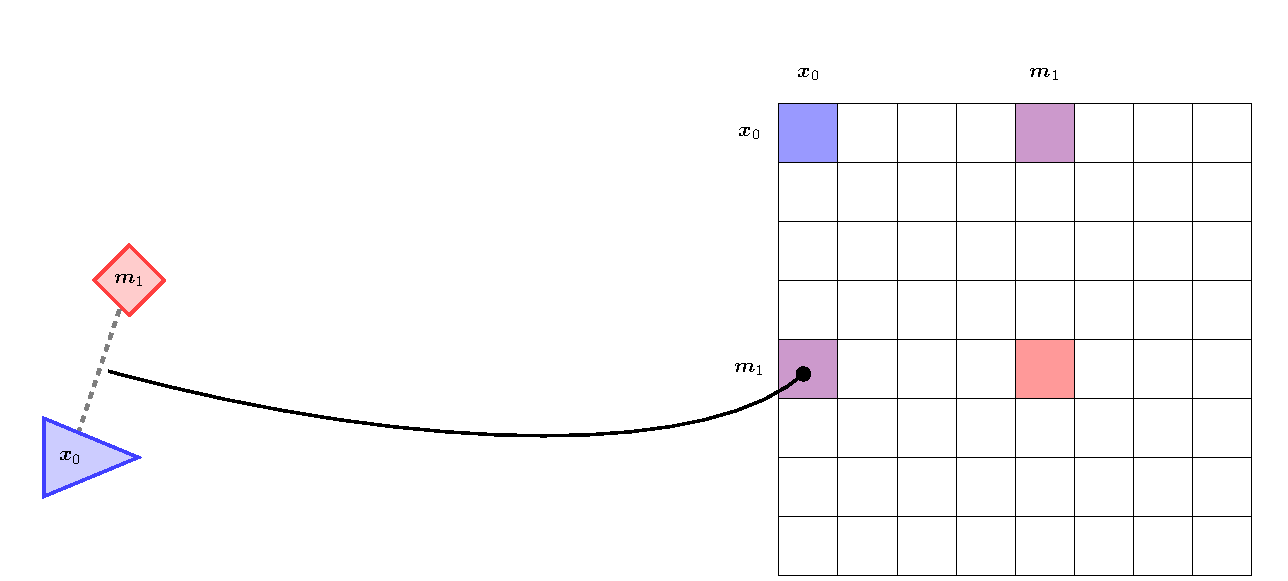
\includegraphics[width=\figScale\textwidth]{tikz/matrix1.pdf}
        \caption{Block addition to the information matrix after a landmark measurement.}
        \label{fig:matrix1}
    \end{subfigure}
    \begin{subfigure}[htbp!]{\textwidth}
        \centering
        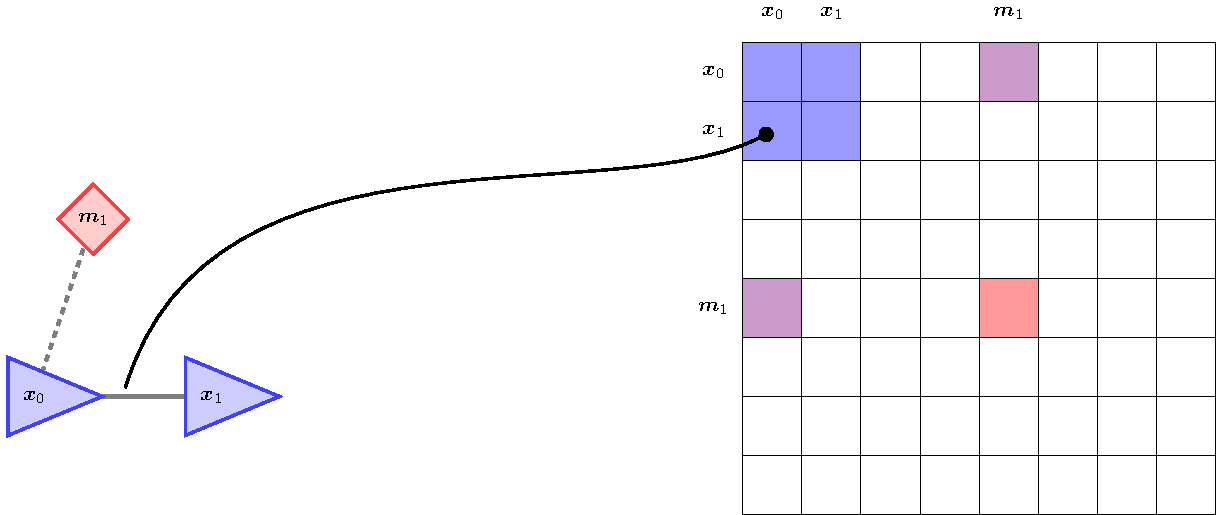
\includegraphics[width=\figScale\textwidth]{tikz/matrix2.pdf}
        \caption{Block addition to the information matrix after a robot movement.}
        \label{fig:matrix2}
    \end{subfigure}
    \begin{subfigure}[htbp!]{\textwidth}
        \centering
        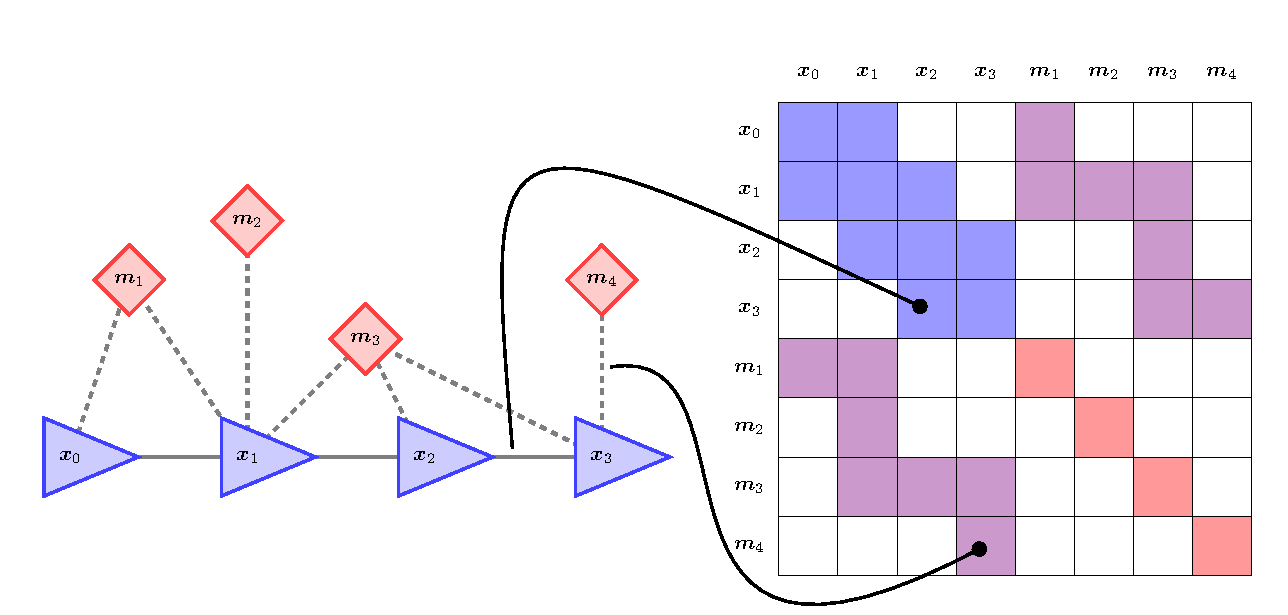
\includegraphics[width=\figScale\textwidth]{tikz/matrix3-cropped.pdf}
        \caption{Shows the block structure of the information matrix after 3 robot movements and 7 measurement.}
        \label{fig:matrix3}
    \end{subfigure}
    \caption[Information matrix structure]{Progressing filling of the information matrix as the robot moves and takes measurements. Blue: pose-pose block. Purple: pose-landmark block. Red: landmark-landmark block.}
    \label{fig:information-matrix}
\end{figure}

The information matrix can be divided in four submatrices. The top-left matrix (filled with blue squares) has the relative information between to pair of poses. Since the information acquired is only relative to two consecutive poses, 
this submatrix has a band diagonal structure, leaving all the other elements in zero. The top-right and bottom-left submatrices are equivalent, and contains the relative information between a pose and a measured landmark. The number of block in these matrices depends on the number of landmarks measured, but is often in SLAM that only spatially close landmark are measured at every pose, leaving these matrices, again, with much of their elements in zero. Finally, the bottom-right submatrix regards information about pair of landmarks. Since there are not direct measurement between two landmarks, this submatrix is leaved as a block diagonal matrix.

Therefore it's shown that the number of non-zero elements in $\bs{H}$ is proportional to the number of edges in the graph, leading to a matrix with a large number of zero elements. Tis kind of matrices are called \it{sparse matrices}. Fast and efficient algorithm exist to solve~\eqref{eq:linear-system} for sparse matrices, such as Cholesky decomposition and Preconditioned Conjugate Gradient (PCG). These algorithms are already implemented in the g$^2$o framework that will be used.

\subsection{Review of the State of the Art in SLAM}
\label{sec:state-of-the-art}

SLAM as a probabilistic problem has its beginning in the 1986 IEEE Robotics and Automation Conference held in San Francisco, California~\cite{tutorial}. One of the first papers to give a solution to SLAM was \cite{ekfslam} using the Extended Kalman Filter technique. This solution is now known EKF SLAM.

One of the first papers to state SLAM as an optimization over a graph is~\cite{firstgraph} by Li and Milios. They were the first to treat motion and measurement in a equally as information constrains, which differed form standard EKF view where motion information is used for prediction, and measurement as correction for the Kalman filter.

The GraphSLAM algorithm as stated in the work was first presented in~\cite{graphslam} by Thrun and Montemerlo. In this paper the SLAM negative likelihood posterior is derived for solving the full SLAM problem, and the optimization problem is stated in a similar way as in section~\ref{sec:graphslam-description}. However, it not specify the way of solving the optimization in~\eqref{eq:minimization}. 

From there, several improvement have been made to the general idea of the GraphSLAM algorithm. In~\cite{sqrtsam} a similar graph representation is used to solve SLAM, called $\sqrt{\text{SAM}}$, but it used a \it{smoothing} approach, meaning that the entire robot trajectory up to the current time is estimated. They implement a batch and incremental algorithm for SLAM solving, and use either QR or Cholesky factorization of the linear equation solving, with variable ordering for complexity improvement. 

An updated version of $\sqrt{\text{SAM}}$, called iSAM, is presented in~\cite{isam}. It improves the performance in the incremental version, by directly updating the square root information matrix with new measurement as they arrive. It also avoid unnecessary fill-in int information matrix generated by trajectory loop, by doing periodic variable reordering. It solves online data association using maximum likelihood and nearest neighbor matching.

Another improvement of iSAM is presented in~\cite{isam2}, iSAM2, in which they define a new data structure, called \it{Bayes Tree}, that allows them to improve the performance in the online case, by updating only the necessary variables in the linearization point after arrival of new data. 

In~\cite{robustloop} a robust consistency-based loop-closure verification method, Realizing, Reversing, and Recovering (RRR) algorithm, is presented for de detection and correction of incorrect loop closure generated by the SLAM algorithm. Incorrect loop closure appear when a robot visit similar looking locations, and can severely corrupt the map estimate.     

For efficiently solving graph optimization problems that appear in SLAM and other situations, a framework called g$^2$o (general graph optimization) is presented in~\cite{g2o}. g$^2$o is an open source optimization tool written in \verb!C++!.  It was designed to be easily extensible to a wide range of problems, and it contains typical optimization techniques used for sparse matrices, such as Cholesky decomposition and Preconditioned Conjugate Gradient. 

The contribution of this \mem{} is to provide a fully functional GraphSLAM algorithm, which could be used for the navigation of robots in real world scenarios, and for the realization of comparative analysis with other SLAM algorithms.